\documentclass[10pt]{amsart}
\usepackage[a4paper,margin=23mm]{geometry}
\usepackage{amsmath,amssymb,amsthm,graphicx,hyperref,etoolbox,dsfont,xcolor}
\usepackage[shortlabels]{enumitem}
\usepackage{float}
\usepackage{tikz}\usetikzlibrary{positioning,arrows,matrix,chains,shadows,shapes}
\usepackage[english]{babel}
\newcommand{\ie}{i.e.}\newcommand{\eg}{e.g.}\newcommand{\resp}{resp.}\newcommand{\cf}{cf.}\newcommand{\skpt}{\par\smallskip\noindent}
\newtheorem{theorem}{Theorem}[section]
\newtheorem{proposition}[theorem]{Proposition}\newtheorem{lemma}[theorem]{Lemma}\newtheorem{corollary}[theorem]{Corollary}
\theoremstyle{definition}\newtheorem{definition}[theorem]{Definition}\newtheorem{remark}[theorem]{Remark}\newtheorem{example}[theorem]{Example}
\emergencystretch=3em\pagestyle{plain}
% math special letters
\newcommand{\R}{\mathbb{R}} % reals
\newcommand{\N}{\mathbb{N}} % naturals
\newcommand{\Z}{\mathbb{Z}} % integers
\newcommand{\C}{\mathbb{C}} % complex
\newcommand{\I}{\mathbb{I}} % set of integers
\newcommand{\HH}{\mathbb{H}} % hyperplane
\newcommand{\fA}{\mathfrak{A}} % alternating group
\newcommand{\fS}{\mathfrak{S}} % symmetric group
\newcommand{\fP}{\mathfrak{P}} % partitions
\newcommand{\cC}{\mathcal{C}} % circle
\newcommand{\fX}{\mathfrak{X}} % generating function
\renewcommand{\b}[1]{\mathbf{#1}} % bold letters

% math commands
\newcommand{\set}[2]{\left\{ #1 \;\middle|\; #2 \right\}} % set notation
\newcommand{\bigset}[2]{\big\{ #1 \;|\; #2 \big\}} % big set notation
\newcommand{\biggset}[2]{\bigg\{ #1 \;\bigg|\; #2 \bigg\}} % bigg set notation
\newcommand{\ssm}{\smallsetminus} % small set minus
\newcommand{\dotprod}[2]{\langle \, #1 \; | \; #2 \, \rangle} % dot product
\newcommand{\symdif}{\,\triangle\,} % symmetric difference
\newcommand{\one}{{1\!\!1}} % the all one vector
\newcommand{\eqdef}{\mbox{\,\raisebox{0.2ex}{\scriptsize\ensuremath{\mathrm:}}\ensuremath{=}\,}} % :=
\newcommand{\defeq}{\mbox{~\ensuremath{=}\raisebox{0.2ex}{\scriptsize\ensuremath{\mathrm:}} }} % =:
\newcommand{\polar}{^\diamond} % polar
\newcommand{\blackPolar}{^\blacklozenge} % black polar
\newcommand{\simplex}{\triangle} % simplex
\newcommand{\binomspec}[3]{\begin{pmatrix} #1 \\ #2 \end{pmatrix}_{\!\!#3}} % special binomial coefficient (ou {\begin{Bmatrix} #1 \\ #2 \end{Bmatrix}_{#3})
\renewcommand{\implies}{\Rightarrow} % imply sign
\newcommand{\sep}{|} % separation for ordered partitions
\newcommand{\freeSep}{\freeGap\hspace{-.92mm}|} % free separation for ordered partitions
\newcommand{\bsep}{\,|\,} % big separation for ordered partitions
\newcommand{\Id}{\mathrm{Id}} % identity
\newcommand{\sign}{\mathrm{sign}} % sign

% trees
\newcommand{\graphG}[1][G]{\mathrm{#1}} % graph
\newcommand{\tree}[1][T]{\mathrm{#1}} % tree
\newcommand{\ground}{\mathrm{V}} % vertex set
\newcommand{\decoration}{\delta} % decoration of a Cambrian tree
\newcommand{\Decorations}{\{\noneCirc{}, \downCirc{}, \upCirc{}, \upDownCirc{}\}} % all decorations
\newcommand{\less}{\preccurlyeq} % refinement order on decorations
\newcommand{\pdecoration}{\decoration_p} % p-decoration of a decorated permutation
\newcommand{\vdecoration}{\decoration_v} % v-decoration of a decorated permutation
\newcommand{\generatingTree}{\mathcal{T}} % generating tree of permutations avoiding the two Cambrian patterns
\newcommand{\generatingTreeSchroder}{\mathcal{S}} % generating tree of permutations avoiding the two Cambrian patterns
\newcommand{\level}{m} % level in generating tree
\newcommand{\up}[1]{\overline{#1}}
\newcommand{\upr}[1]{{\red \up{#1}}}
\newcommand{\upb}[1]{{\blue \up{#1}}}
\newcommand{\down}[1]{\underline{#1}}
\newcommand{\downr}[1]{{\red \down{#1}}}
\newcommand{\downb}[1]{{\blue \down{#1}}}
\newcommand{\updown}[1]{\up{\down{#1}}}
\newcommand{\updownr}[1]{{\red \updown{#1}}}
\newcommand{\updownb}[1]{{\blue \updown{#1}}}
\newcommand{\linearExtensions}{\mathcal{L}} % linear extensions
\newcommand{\circDecoration}{{\text{\tiny$\bigcirc$}}} % small blue circle
\newcommand{\squareDecoration}{{\text{\raisebox{-.05cm}{$\square$}}}} % small red square
\newcommand{\edgecut}[2]{\left( #1 \;\middle\|\; #2 \right)} % edge cut
\newcommand{\cuts}{\mathsf{EC}} % edge cuts
\newcommand{\decreasingCuts}{\mathsf{DEC}} % decreasing edge cuts
\newcommand{\dash}{\text{-}}
\newcommand{\Permutrees}{\mathcal{PT}} % permutrees
\newcommand{\SchrPermutrees}{\mathrm{SchrPT}} % Schroder-permutrees
\newcommand{\factCatalan}[1]{\text{\bf C}(#1)} % factorial-Catalan number
\newcommand{\factSchroder}[1]{\text{\bf S}(#1)} % factorial Schroder number

% arc diagrams
\newcommand{\arcDiagrams}{\mathcal{A}} % arc diagrams
\newcommand{\asc}{\mathsf{asc}} % ascent bijection from permutations to arc diagrams
\newcommand{\desc}{\mathsf{desc}} % descent bijection from permutations to arc diagrams

% Polytopes
\newcommand{\Perm}[1][n]{\mathds{P}\mathrm{erm}(#1)} % permutahedron
\newcommand{\Asso}[1][n]{\mathds{A}\mathrm{sso}(#1)} % associahedron
\newcommand{\Para}[1][n]{\mathds{P}\mathrm{ara}(#1)} % parallelepiped
\newcommand{\Zono}[1][\decoration]{\mathds{Z}\mathrm{ono}(#1)} % zonotope
\newcommand{\Permutreehedron}[1][\decoration]{\mathds{PT}(#1)} % permutreehedron
\newcommand{\Cone}{\mathrm{C}} % cone
\newcommand{\fan}{\mathcal{F}} % fan
\newcommand{\Fan}[1][\decoration]{\fan(#1)} % permutree fan
\newcommand{\Hyp}{\b{H}^=} % hyperplane
\newcommand{\HS}{\b{H}^\ge} % half-space
\newcommand{\face}{\mathsf{F}} % face

% operators
\DeclareMathOperator{\conv}{conv} % convex hull
\DeclareMathOperator{\cone}{cone} % cone hull
\DeclareMathOperator{\coinv}{coinv} % coinversion set
\newcommand{\meet}{\wedge} % meet in lattice
\newcommand{\join}{\vee} % join in lattice
\newcommand{\projDown}{\pi_{\!\downarrow\!}} % down projection lattice congruence
\newcommand{\projUp}{\pi^{\!\uparrow\!}} % up projection lattice congruence
\newcommand{\verticalSymmetry}[1]{#1^{\;\mathbin{\tikz [thin, baseline=-0.2em] \draw [<->] (0em,-.3em) -- (0em,.3em);}}\,} % vertical symmetry of permutrees
\newcommand{\horizontalSymmetry}[1]{#1^{\mathbin{\tikz [baseline=-0.2em] \draw [<->] (-.3em,0em) -- (.3em,0em);}}} % horizontal symmetry of permutrees
\newcommand{\horizontalVerticalSymmetry}[1]{#1^{\mathbin{\tikz [baseline=-0.2em] {\draw [<->] (0em,-.3em) -- (0em,.3em); \draw [<->] (-.4em,0em) -- (.4em,0em);}}}} % horizontal and vertical symmetry of permutrees

% Hopf algebras
\newcommand{\FQSym}{\mathsf{FQSym}} % quasi-symmetric functions
\newcommand{\PBT}{\mathsf{PBT}} % PBT (Loday-Ronco)
\newcommand{\PermutreeAlgebra}{\mathsf{PT}} % Permutree Algebra
\newcommand{\SchrPermutreeAlgebra}{\mathsf{SchrPT}} % Schroder-Permutree Algebra
\newcommand{\OrdPart}{\mathsf{OrdPart}} % ordered partition Hopf algebra
\newcommand{\sfx}{\mathsf{x}} % element of Alg
\newcommand{\sfy}{\mathsf{y}} % element of Alg
\newcommand{\sfz}{\mathsf{z}} % element of Alg
\newcommand{\integerPointTransform}{\mathbb{Z}} % integer point transform

% operations
\newcommand{\product}{\cdot} % product
\newcommand{\coproduct}{\triangle} % coproduct
\newcommand{\shiftedShuffle}{\,\bar\shuffle\,} % shifted shuffle
\newcommand{\convolution}{\star} % shifted shuffle
\newcommand{\underprod}[2]{{#1}\backslash{#2}} % #1 under #2
\newcommand{\overprod}[2]{{#1}\slash{#2}} % #1 over #2

% bases
\newcommand{\F}{\mathbb{F}} % F-basis of FQSym
\newcommand{\G}{\mathbb{G}} % G-basis of FQSym
\newcommand{\HFQSym}{\mathbb{H}} % H-basis of FQSym
\newcommand{\EFQSym}{\mathbb{E}} % E-basis of FQSym
\newcommand{\PPT}{\mathbb{P}} % P-basis of PT
\newcommand{\QPT}{\mathbb{Q}} % Q-basis of PT*
\newcommand{\HPT}{\mathbb{H}} % H-basis of PT
\newcommand{\EPT}{\mathbb{E}} % E-basis of PT

% correspondences
\newcommand{\permutreeCorresp}{\Theta} % bijection from the permutations to the leveled permutrees
\newcommand{\SchroderPermutreeCorresp}{\Theta^\star} % bijection from the permutations to the leveled Schroder permutrees
\NewDocumentCommand{\surjection}{O{\decoration} O{\decoration'}}{\Psi_{#1}^{#2}} % surjection from #1-permutrees to #2-permutrees
\NewDocumentCommand{\surjectionSchroder}{O{\decoration} O{\decoration'}}{{\Psi^\star}_{#1}^{#2}} % surjection from #1-permutrees to #2-permutrees
\newcommand{\PSymbol}{\mathbf{P}} % P-symbol
\newcommand{\QSymbol}{\mathbf{Q}} % Q-symbol
\newcommand{\SchroderPSymbol}{\mathbf{P}^\star} % Schroder P-symbol

% others
\newcommand{\fref}[1]{Figure~\ref{#1}} % reference figures
\renewcommand{\ie}{\textit{i.e.}~} % id est
\renewcommand{\eg}{\textit{e.g.}~} % exempli gratia
\definecolor{darkblue}{rgb}{0,0,0.7} % darkblue color
\newcommand{\darkblue}{\color{darkblue}} % darkblue command
\newcommand{\red}{\color{red}} % red command
\newcommand{\blue}{\color{blue}} % blue command
\newcommand{\defn}[1]{\emph{\darkblue #1}} % emphasis of a definition
\usepackage{todonotes}
\newcommand{\noneCirc}{\ensuremath{\mathchoice{\raisebox{-.7mm}{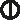
\includegraphics[height=2.2ex]{assets/none.pdf}}}{\raisebox{-.7mm}{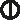
\includegraphics[height=2.2ex]{assets/none.pdf}}}{\raisebox{-.6mm}{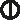
\includegraphics[height=1.6ex]{assets/none.pdf}}}{\raisebox{-.5mm}{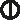
\includegraphics[height=1ex]{assets/none.pdf}}}}}
\newcommand{\downCirc}{\ensuremath{\mathchoice{\raisebox{-.7mm}{
\includegraphics[height=2.2ex]{assets/down.pdf}}}{\raisebox{-.7mm}{
\includegraphics[height=2.2ex]{assets/down.pdf}}}{\raisebox{-.6mm}{
\includegraphics[height=1.6ex]{assets/down.pdf}}}{\raisebox{-.5mm}{
\includegraphics[height=1ex]{assets/down.pdf}}}}}
\newcommand{\upCirc}{\ensuremath{\mathchoice{\raisebox{-.7mm}{
\includegraphics[height=2.2ex]{assets/up.pdf}}}{\raisebox{-.7mm}{
\includegraphics[height=2.2ex]{assets/up.pdf}}}{\raisebox{-.6mm}{
\includegraphics[height=1.6ex]{assets/up.pdf}}}{\raisebox{-.5mm}{
\includegraphics[height=1ex]{assets/up.pdf}}}}}
\newcommand{\upDownCirc}{\ensuremath{\mathchoice{\raisebox{-.7mm}{
\includegraphics[height=2.2ex]{assets/updown.pdf}}}{\raisebox{-.7mm}{
\includegraphics[height=2.2ex]{assets/updown.pdf}}}{\raisebox{-.6mm}{
\includegraphics[height=1.6ex]{assets/updown.pdf}}}{\raisebox{-.5mm}{
\includegraphics[height=1ex]{assets/updown.pdf}}}}}
\makeatletter
\expandafter\def\csname sourcefig@fig:leveledPermutree\endcsname{2}
\expandafter\def\csname sourcefig@fig:insertionAlgorithm\endcsname{6}
\expandafter\def\csname sourcefig@fig:permutreehedra\endcsname{16}
\renewcommand{\fref}[1]{\ifcsname sourcefig@#1\endcsname\href{https://doi.org/10.5802/alco.1}{Figure \csname sourcefig@#1\endcsname\ of the source article}\else Figure~\ref{#1}\fi}
\makeatother
\begin{document}
\title{Permutree fans are normal fans of explicit deleted-inequality permutreehedra for arbitrary four-type decorations}
\author{Vincent Pilaud \and Viviane Pons}
\maketitle
\setcounter{section}{1}
\section{Permutree source definitions and correspondence}
\begin{definition}
\label{def:permutree}
A \defn{permutree} is a directed tree~$\tree$ with vertex set~$\ground$ endowed with a bijective vertex labeling $p : \ground \to [n]$ such that for each vertex~$v \in \ground$,
\begin{enumerate}[(i)]
\item $v$ has one or two parents (outgoing neighbors), and one or two children (incoming neighbors);
\item if $v$ has two parents (resp.~children), then all labels in the left ancestor (resp. descendant) subtree of~$v$ are smaller than~$p(v)$ while all labels in the right ancestor (resp.~descendant) subtree of~$v$ are larger than~$p(v)$.
\end{enumerate}
The \defn{decoration} of a permutree is the $n$-tuple~$\decoration(\tree) \in \Decorations^n$ defined by
\[
\decoration(\tree)_{p(v)} = 
\begin{cases}
\noneCirc{} & \text{if $v$ has one parent and one child,} \\
\downCirc{} & \text{if $v$ has one parent and two children,} \\
\upCirc{} & \text{if $v$ has two parents and one child,} \\
\upDownCirc{} & \text{if $v$ has two parents and two children,}
\end{cases}
\]
for all~$v \in \ground$. Equivalently, we record the \defn{up} labels~${\decoration^\vee(\tree) = \set{i \in [n]}{\decoration(\tree)_i \in \{\upCirc{},\upDownCirc{}\}}}$ of vertices with two parents and the \defn{down} labels~$\decoration_\wedge(\tree) = \set{i \in [n]}{\decoration(\tree)_i \in \{\downCirc{},\upDownCirc{}\}}$ of vertices with two children. If~$\decoration(\tree) = \decoration$, we say that $\tree$ is a \defn{$\decoration$-permutree}. 

We denote by~$\Permutrees(\decoration)$ the set of $\decoration$-permutrees, by~$\Permutrees(n) = \bigsqcup_{\decoration \in \Decorations^n} \Permutrees(\decoration)$ the set of all permutrees on~$n$ vertices, and by~$\Permutrees \eqdef \bigsqcup_{n \in \N} \Permutrees(n)$ the set of all permutrees.
\end{definition}

\begin{definition}
\label{def:increasingTree}
An \defn{increasing tree} is a directed tree~$\tree$ with vertex set~$\ground$ endowed with a bijective vertex labeling~$q : \ground \to [n]$ such that~$v \to w$ in~$\tree$ implies~$q(v) < q(w)$.
\end{definition}

\begin{definition}
\label{def:labeledPermutree}
A \defn{leveled permutree} is a directed tree~$\tree$ with vertex set~$\ground$ endowed with two bijective vertex labelings~${p,q : V \to [n]}$ which respectively define a permutree and an increasing tree. In other words, a leveled permutree is a permutree endowed with a linear extension of its transitive closure (given by the inverse of the labeling~$q$).
\end{definition}
\fref{fig:leveledPermutree} provides examples of a permutree, an increasing tree, and a leveled permutree. We use the following conventions in all figures of this paper:
\begin{enumerate}[(i)]
\item All edges are oriented bottom-up --- we can thus omit the edge orientation;
\item For a permutree, the vertices appear from left to right in the order given by the labeling~$p$ --- we can thus omit the vertex labeling;
\item For an increasing tree, the vertices appear from bottom to top in the order given by the labeling~$q$ --- we can thus omit the vertex labeling;
\item In particular, for a leveled permutree with vertex labelings~$p,q : \ground \to [n]$ as in Definition~\ref{def:labeledPermutree}, each vertex~$v$ appears at position~$\big( p(v),q(v) \big)$ --- we can thus omit both labelings;
\item In all our trees, we decorate the vertices with \noneCirc{}, \downCirc{}, \upCirc{}, or \upDownCirc{} depending on their number of parents and children, following the natural visual convention of Definition~\ref{def:permutree};
\item In a permutree, we often draw a vertical red wall below \downCirc{} and \upDownCirc{} vertices and above \upCirc{} and \upDownCirc{} vertices to mark the separation between the left and right descendant or ancestor subtrees of these vertices.
\end{enumerate}
\subsection{Permutree correspondence}
\label{subsec:correspondence}

In this section, we present a correspondence between the permutations of~$\fS_n$ and the leveled $\decoration$-permutrees for any given decoration~$\decoration \in \Decorations$. This correspondence defines a surjection from the permutations of~$\fS_n$ to the $\decoration$-permutrees by forgetting the increasing labeling. This surjection will be a special case of the surjections described in Section~\href{https://doi.org/10.5802/alco.1}{2.7 of the source article}. We follow here the presentation of the Cambrian correspondence in~\cite{ChatelPilaud}.

We represent graphically a permutation~$\tau \in \fS_n$ by the $(n \times n)$-table, with rows labelled by positions from bottom to top and columns labelled by values from left to right, and with a dot at row~$i$ and column~$\tau(i)$ for all~$i \in [n]$. (This unusual choice of orientation is necessary to fit later with the existing constructions of~\cite{LodayRonco, HivertNovelliThibon-algebraBinarySearchTrees, ChatelPilaud}.)

A \defn{decorated permutation} is a permutation table where each dot is decorated by~\noneCirc{}, \downCirc{}, \upCirc{},~or~\upDownCirc{}. See the top left corner of \fref{fig:insertionAlgorithm}. We could equivalently think of a permutation where the positions or the values receive a decoration, but it will be useful later to switch the decoration from positions to values. The \defn{p-decoration} (resp.~\defn{v-decoration}) of a decorated permutation~$\tau$ is the sequence~$\pdecoration(\tau)$ (resp.~$\vdecoration(\tau)$) of decorations of~$\tau$ ordered by positions from bottom to top (resp.~by values from left to right). For a permutation~$\tau \in \fS_n$ and a decoration~$\decoration \in \Decorations^n$, we denote by~$\tau_\decoration$ (resp.~by~$\tau^\decoration$) the permutation~$\tau$ with p-decoration~$\pdecoration(\tau_\decoration) = \decoration$ (resp.~with \mbox{v-decoration}~$\vdecoration(\tau^\decoration) = \decoration$). We let~$\fS_\decoration \eqdef \set{\tau_\decoration}{\tau \in \fS_n}$ and~$\fS^\decoration \eqdef \set{\tau^\decoration}{\tau \in \fS_n}$. Finally, we let
\[
\fS_{\Decorations} \eqdef \bigsqcup_{\substack{n \in \N \\ \decoration \in \Decorations^n}} \fS_\decoration = \bigsqcup_{\substack{n \in \N \\ \decoration \in \Decorations^n}} \fS^\decoration
\]
denote the set of all decorated permutations.

In concrete examples, we underline the down positions/values (those decorated by~\downCirc{} or~\upDownCirc{}) while we overline the up positions/values (those decorated by~\upCirc{} or~\upDownCirc{}): for example, $\up{2}\up{7}5\down{1}3\updown{4}\down{6}$ is the decorated permutation represented on the top left corner of \fref{fig:insertionAlgorithm}, where~${\tau = [2,7,5,1,3,4,6]}$, ${\pdecoration = \upCirc{}\upCirc{}\noneCirc{}\downCirc{}\noneCirc{}\upDownCirc{}\downCirc{}}$ and~${\vdecoration = \downCirc{}\upCirc{}\noneCirc{}\upDownCirc{}\noneCirc{}\downCirc{}\upCirc{}}$.

The insertion algorithm transforms a decorated permutation~$\tau$ to a leveled permutree~$\permutreeCorresp(\tau)$. As a preprocessing, we represent the table of~$\tau$ (with decorated dots in positions~$(\tau(i),i)$ for~$i \in [n]$) and draw a vertical red wall below the down vertices and above the up vertices. These walls separate the table into regions. Note that the number of children (resp. parents) expected at each vertex is the number of regions visible below (resp. above) this vertex. We then sweep the table from bottom to top (thus reading the permutation~$\tau$ from left to right) as follows. The procedure starts with an incoming strand in between any two consecutive down values. At each step, we sweep the next vertex and proceed to the following operations depending on its decoration:
\begin{enumerate}[(i)]
\item a vertex decorated by \noneCirc{} or \upCirc{} catches the only incoming strands it sees, while a vertex decorated by \downCirc{} or \upDownCirc{} connects the two incoming strands just to its left and to its~right,
\item a vertex decorated by \noneCirc{} or \downCirc{} creates a unique outgoing strand, while a vertex decorated by \upCirc{} or \upDownCirc{} creates two outgoing strands just to its left and to its right.
\end{enumerate}
The procedure finishes with an outgoing strand in between any two consecutive up values. See \fref{fig:insertionAlgorithm}.
\begin{proposition}
\label{prop:permutreeCorrespondence}
The map~$\permutreeCorresp$ is a bijection from $\decoration$-decorated permutations to leveled $\decoration$-permutrees.
\end{proposition}

\begin{proof}
First, we need to prove that the map~$\permutreeCorresp$ is well-defined. This relies on the following invariant of the sweeping algorithm: along the sweeping line, there is precisely one strand in each of the intervals separated by the walls. Indeed, this invariant  holds when we start the procedure and is preserved when we sweep any kind of vertex. Therefore, the sweeping algorithm creates a graph whose vertices are the decorated dots of the permutation table together with the initial and final positions of the strands and where no edge crosses a red wall. It follows that this graph is a tree (a cycle would force an edge to cross a red wall), and it is a leveled permutree (the walls separate left and right ancestor or descendant subtrees). To prove that~$\permutreeCorresp$ is bijective, we already observed that a leveled permutree~$\tree$ is a permutree endowed with a linear extension~$\tau$. We can consider that~$\tau$ is decorated by the decorations of the vertices of~$\tree$. Finally, one checks easily that when inserting the decorated permutation~$\tau$, the resulting leveled permutree is~$\permutreeCorresp(\tau) = \tree$.
\end{proof}

For a decorated permutation~$\tau$, we denote by~$\PSymbol(\tau)$ the permutree obtained by forgetting the increasing labeling in~$\permutreeCorresp(\tau)$ and by~$\QSymbol(\tau)$ the increasing tree obtained by forgetting the permutree labeling in~$\permutreeCorresp(\tau)$. These trees should be thought of as the insertion and recording trees of the permutree correspondence, in analogy to the insertion and recording tableaux in the Robinson-Schensted correspondence~\cite{Schensted}. The same analogy was already done for the sylvester correspondence~\cite{HivertNovelliThibon-algebraBinarySearchTrees} and the Cambrian correspondence~\cite{ChatelPilaud}. The following statement was already observed along the previous proof.

\begin{proposition}
\label{prop:fibersPSymbol}
The decorated permutations~$\tau \in \fS^\decoration$ such that~$\PSymbol(\tau) = \tree$ are precisely the linear extensions of (the transitive closure of) the permutree~$\tree$.
\end{proposition}
\begin{definition}
\label{def:permutreeCongruence}
For a decoration~$\decoration \in \Decorations^n$, the \defn{$\decoration$-permutree congruence} is the equivalence relation on~$\fS^\decoration$ defined as the transitive closure of the rewriting rules
\[
\begin{array}{ll}
UacVbW \equiv_\decoration UcaVbW & \text{if } a < b < c \text{ and } \decoration_b = \downCirc{} \text{ or } \upDownCirc{}, \\
UbVacW \equiv_\decoration UbVcaW & \text{if } a < b < c \text{ and } \decoration_b = \upCirc{} \text{ or } \upDownCirc{},
\end{array}
\]
where~$a,b,c$ are elements of~$[n]$ while~$U,V,W$ are words on~$[n]$. Note that the decorations of~$a$ and~$c$ do not matter, only that of~$b$ which we call the \defn{witness} of the rewriting rule.

The \defn{permutree congruence} is the equivalence relation on all decorated permutations~$\fS_{\Decorations}$ obtained as the union of all $\decoration$-permutree congruences:
\[
\equiv \; \eqdef \bigsqcup_{\substack{n \in \N \\ \decoration \in \Decorations^n}} \!\! \equiv_\decoration.
\]
\end{definition}

\begin{proposition}
\label{prop:permutreeCongruenceClass}
Two decorated permutations~$\tau, \tau' \in \fS_{\Decorations}$ are permutree congruent if and only if they have the same $\PSymbol$-symbol:
\[
\tau \equiv \tau' \iff \PSymbol(\tau) = \PSymbol(\tau').
\]
\end{proposition}

\begin{proof}
It boils down to observe that two consecutive vertices~$a,c$ in a linear extension~$\tau$ of a \mbox{$\decoration$-permu}\-tree~$\tree$ can be switched while preserving a linear extension~$\tau'$ of~$\tree$ precisely when they belong to distinct ancestor or descendant subtrees of a vertex~$b$ of~$\tree$. It follows that the vertices~$a,c$ lie on either sides of~$b$ so that we have~$a < b < c$. If~$\decoration_b = \downCirc{}$ or~$\upDownCirc{}$ and~$a,c$ appear before~$b$ in~$\tau$, then they belong to distinct descendant subtrees of~$b$ and~$\tau = UacVbW$ can be switched to~$\tau' = UcaVbW$. If~$\decoration_b = \upCirc{}$ or~$\upDownCirc{}$ and~$a,c$ appear after~$b$ in~$\tau$, then they belong to distinct ancestor subtrees of~$b$ and~$\tau = UbVacW$ can be switched to~$\tau' = UbVcaW$.
\end{proof}
\subsection{Rotations and permutree lattices}
\label{subsec:rotations}

We now extend the rotation from binary trees to all permutrees. This local operation only exchanges the orientation of an edge and rearranges the endpoints of two other edges.

\begin{definition}
\label{def:rotation}
Let~$i \to j$ be an edge in a $\decoration$-permutree~$\tree$, with~$i < j$. Let~$D$ be the only (resp. the right) descendant subtree of vertex~$i$ if~${\decoration_i \in \{\noneCirc{}, \upCirc{}\}}$ (resp.~${\decoration_i \in \{\downCirc{}, \upDownCirc{}\}}$) and let~$U$ denote the only (resp.~the left) ancestor subtree of vertex~$j$ if~$\decoration_j \in \{\noneCirc{}, \downCirc{}\}$ (resp.~$\decoration_j \in \{\upCirc{}, \upDownCirc{}\}$). Let~$\tree'$ be the oriented tree obtained from~$\tree$ just reversing the orientation of~$i \to j$ and attaching the subtree~$U$ to~$i$ and the subtree~$D$ to~$j$. The transformation from~$\tree$ to~$\tree'$ is called \defn{rotation} of the edge~$i \to j$. See \fref{fig:rotation}.

\medskip

\begin{figure}[H]%%Fig 9
  \centerline{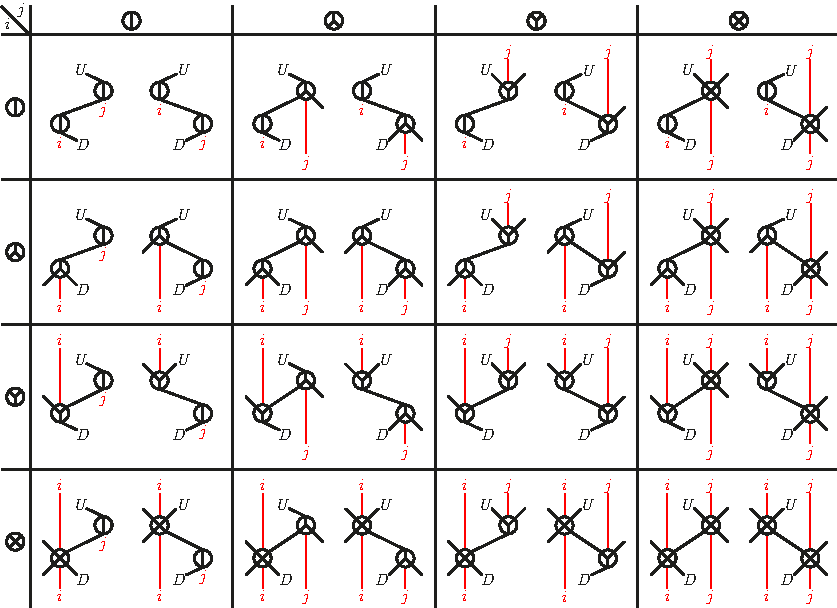
\includegraphics[scale=.8]{assets/rotation.pdf}}
  \caption{Rotations in permutrees: in each box, the tree~$\tree$ (left) is transformed into the tree~$\tree'$ (right) by rotation of the edge~$i \to j$. The $16$ boxes correspond to the possible decorations of~$i$~and~$j$.}
  \label{fig:rotation}
\end{figure}
\end{definition}
\par\smallskip\noindent Original Figure~9 labels: the row is $i$ and the column is $j$; their decoration labels, in order, are $\noneCirc{},\downCirc{},\upCirc{},\upDownCirc{}$.
Each tree has vertex labels $i,j$ and subtree labels $U,D$. The four decoration meanings and the subtrees $U,D$ are given in the editable definitions above.
The following statement shows that the rotation of the edge~$i \to j$ is the only operation which exchanges the orientation of this edge while preserving all other edge cuts. An \defn{edge cut} in a permutree~$\tree$ is the ordered partition~$\edgecut{I}{J}$ of the vertices of~$\tree$ into the set~$I$ of vertices in the source set and the set~$J = [n] \ssm I$ of vertices in the target set of an oriented edge of~$\tree$.

\begin{proposition}
\label{prop:rotation}
The result~$\tree'$ of the rotation of an edge~$i \to j$ in a $\decoration$-permutree~$\tree$ is a \mbox{$\decoration$-permutree}. Moreover, $\tree'$ is the unique $\decoration$-permutree with the same edge cuts as~$\tree$, except the cut defined by the edge~$i \to j$.
\end{proposition}

\begin{proof}
We first observe that~$\tree'$ is still a tree, with an orientation of its edges and a bijective labeling of its vertices by~$[n]$. To check that~$\tree'$ is still a $\decoration$-permutree, we need to check the local conditions of Definition~\ref{def:permutree} around each vertex of~$\tree'$. Since we did not perturb the labels nor the edges incident to the vertices of~$\tree$ distinct from~$i$ and~$j$, it suffices to check the local conditions around~$i$ and~$j$. By symmetry, we only give the arguments around~$i$. We distinguish two cases:
\begin{itemize}
\item If $i$ is an down vertex in~$\tree$ (decorated by~\downCirc{} or~\upDownCirc{}), then~$D$ is the right descendant of~$i$ in~$\tree$, so that all labels in~$D$ are larger than~$i$. Moreover, all labels in the right ancestor and descendant of~$j$ (if any) are larger than~$j$, which is in turn larger than~$i$. It follows that all labels in the right descendant of~$i$ in~$\tree'$ are larger than~$i$. Finally, the left descendant of~$i$ in~$\tree'$ is the left descendant of~$i$ in~$\tree$, so all its labels are still smaller than~$i$.
\item If~$i$ is an up vertex in~$\tree$ (decorated by~\upCirc{} or~\upDownCirc{}), then~$U$ belongs to the right ancestor of~$i$ in~$\tree$, so that all labels in~$U$ are larger than~$i$. It follows that all labels in the right ancestor of~$i$ in~$\tree'$ are larger than~$i$. Finally, the left ancestor of~$i$ in~$\tree'$ is the left ancestor of~$i$ in~$\tree$, so all its labels are still smaller~than~$i$.
\end{itemize}
This closes the proof that~$\tree'$ is a $\decoration$-permutree.
%
By construction, the $\decoration$-permutree~$\tree'$ clearly has the same edge cuts as~$\tree$, except the cut corresponding to the edge~$i \to j$. Any $\decoration$-permutree with this property is obtained from~$\tree$ by reversing the edge~$i \to j$ to an edge~$i \leftarrow j$ and rearranging the neighbors of~$i$ and~$j$. But it is clear that the rearrangement given in Definition~\ref{def:rotation} is the only one which preserves the local conditions of Definition~\ref{def:permutree} around the vertices~$i$ and~$j$.
\end{proof}
\section{The complete fan and its polytopal realization}
\subsection{Permutree fans}
\label{subsec:permutreeFans}

We consider the (type~$A$) Coxeter arrangement defined by the hyperplanes~$\set{\b{x} \in \R^n}{x_i = x_j}$ for all~$1 \le i < j \le n$. It defines a complete simplicial fan, called the \defn{braid fan}. Each maximal cone~$\Cone$ of this fan corresponds to a permutation given by the order of the coordinates of any point of~$\Cone$. More precisely, each permutation~$\tau$ yields the maximal cone~$\Cone\polar(\tau) \eqdef \set{\b{x} \in \R^n}{x_{\tau^{-1}(1)} \le \dots \le x_{\tau^{-1}(n)}}$ of the braid fan.

For a permutree~$\tree$, define now its \defn{incidence cone}~$\Cone(\tree)$ by\begin{align*}
\Cone(\tree)
& \eqdef \frac{n+1}{2}\one + \cone \set{\b{e}_i-\b{e}_j}{\forall\, i \to j \text{ in } \tree} \\
& = \biggset{\b{x} \in \HH}{\sum_{j \in J} \frac{x_j}{|J|} \le \sum_{i \in I} \frac{x_i}{|I|}, \, \forall \edgecut{I}{J} \in \cuts(\tree)}
\end{align*}
and its \defn{braid cone}~$\Cone\polar(\tree)$ by
\begin{align*}
\Cone\polar(\tree)
& \eqdef \set{\b{x} \in \HH}{x_i \le x_j, \, \forall \, i \to j \text{ in } \tree} \\
& = \frac{n+1}{2}\one + \cone \biggset{\sum_{j \in J} \frac{\b{e}_j}{|J|} - \sum_{i \in I} \frac{\b{e}_i}{|I|}}{\forall \edgecut{I}{J} \in \cuts(\tree)},
\end{align*}
where~$\cuts(\tree)$ denotes the set of edge cuts of~$\tree$. Note that these two cones both lie in the space~$\HH$, are simplicial, and are polar to each other. We use these cones to construct the permutree~fan.

\begin{proposition}
\label{prop:permutreeFan}
For any decoration~$\decoration \in \Decorations^n$, the collection of cones $\set{\Cone\polar(\tree)}{\tree \in \Permutrees(\decoration)}$, together with all their faces, forms a complete simplicial fan~$\Fan$ of~$\HH$ called \defn{$\decoration$-permutree fan}.
\end{proposition}

\begin{proof}
The statement is a special case of a general result of N.~Reading~\cite[Theorem~1.1]{Reading-HopfAlgebras}, but we give a direct short proof for the convenience of the reader. A cone~$\Cone\polar(\tree)$ is the union of the cones~$\Cone\polar(\tau)$ over all linear extensions~$\tau$ of~$\tree$. Since the sets of linear extensions of the $\decoration$-permutrees form a partition of~$\fS_n$ ($\decoration$-permutree congruence classes), we already know that the cones~$\Cone\polar(\tree)$ for all~$\tree \in \Permutrees(\decoration)$ are interior disjoint and cover the all space~$\R^n$. Now any $\decoration$-permutree~$\tree$ is adjacent by rotation to~$n$ other $\decoration$-permutrees~$\tree_1, \dots, \tree_n$. If~$\tree_k$ is obtained from~$\tree$ by rotating the edge~$i \to j$ with edge cut~$\edgecut{I}{J}$, it has precisely the same edge cuts as~$\tree$ except the edge cut~$\edgecut{I}{J}$. The cone~$\Cone\polar(\tree_k)$ thus shares all but one ray of~$\Cone\polar(\tree)$. We conclude that each facet of~$\Cone\polar(\tree)$ is properly shared by another cone~$\Cone\polar(\tree')$. Since the cones~$\Cone\polar(\tree)$ for all~$\tree \in \Permutrees(\decoration)$ are interior disjoint, it shows that no such cone can improperly share a (portion of a) facet with~$\Cone\polar(\tree)$. We obtain that all cones intersect properly which concludes the proof that we have a complete simplicial fan.
\end{proof}
\subsection{Permutreehedra}
\label{subsec:permutreehedra}

We now construct the $\decoration$-permutreehedron whose normal fan is the $\decoration$-permutree fan. As for J.-L.~Loday's or C.~Hohlweg and C.~Lange's associahedra~\cite{Loday, HohlwegLange}, our permutreehedra are obtained by deleting certain inequalities in the facet description of the classical permutahedron. We thus first recall the vertex and facet descriptions of this polytope. The \defn{permutahedron}~$\Perm$ is the polytope obtained as
\begin{enumerate}[(i)]
\item either the convex hull of the points~$\b{p}(\tau) \eqdef [\tau^{-1}(i)]_{i \in [n]} \in \R^n$, for all~$\tau \in \fS_n$,
\item or the intersection of the hyperplane~$\HH = \Hyp([n])$ with the half-spaces~$\HS(J)$ for~$\varnothing \ne J \subseteq \ground$, where
\begin{align*}
\Hyp(J) & \eqdef \biggset{\b{x} \in \R^n}{\sum_{j \in J} x_j = \binom{|J|+1}{2}} \\\text{and} \qquad \HS(J) & \eqdef \biggset{\b{x} \in \R^n}{\sum_{j \in J} x_j \ge \binom{|J|+1}{2}}.
\end{align*}
\end{enumerate}
Its normal fan is precisely the braid fan described in the previous section. An illustration of~$\Perm[4]$ is given on the bottom of \fref{fig:permutreehedra}.

From this polytope, we construct the \defn{$\decoration$-permutreehedron}~$\Permutreehedron$, for which we give both vertex and facet descriptions:
\begin{enumerate}[(i)]
\item The vertices of~$\Permutreehedron$ correspond to $\decoration$-permutrees. We associate to a \mbox{$\decoration$-permu}\-tree~$\tree$ a point~$\b{a}(\tree) \in \R^n$ whose coordinates are defined by
\[
\b{a}(\tree)_i =
\begin{cases}
1 + d & \text{if } \decoration_i = \noneCirc{}, \\
1 + d + \down{\ell}\down{r} & \text{if } \decoration_i = \downCirc{}, \\
1 + d - \up{\ell}\up{r} & \text{if } \decoration_i = \upCirc{}, \\
1 + d + \down{\ell}\down{r} - \up{\ell}\up{r} & \text{if } \decoration_i = \upDownCirc{},
\end{cases}
\]
where~$d$ denotes the number of the descendants~$i$ in~$\tree$, $\down{\ell}$ and~$\down{r}$ denote the sizes of the left and right descendant subtrees of~$i$ in~$\tree$ when~$\decoration_i \in \{\downCirc{}, \upDownCirc{}\}$, and $\up{\ell}$ and~$\up{r}$ denote the sizes of the left and right ancestor subtrees of~$i$ in~$\tree$ when~$\decoration_i \in \{\upCirc{}, \upDownCirc{}\}$. Note that~$\b{a}(\tree)$ is independent of the decorations of the first and last vertices of~$\tree$.
%
\item The facets of~$\Permutreehedron$ correspond to the \defn{$\decoration$-building blocks}, that is, to all subsets~$I \subset [n]$ such that there exists a $\decoration$-permutree~$\tree$ which admits~$\edgecut{I}{J}$ as an edge cut. We associate to a $\decoration$-building block~$I$ the hyperplane~$\Hyp(I)$ and the half-space~$\HS(I)$ defined above for the permutahedron. Note that~$\decoration$-building blocks are easy to compute on the dual representation described in Remark~\href{https://doi.org/10.5802/alco.1}{2.7 of the source article}: any internal arc~$\alpha$ in~$\b{P}_\decoration$ corresponds to the building block~$I_\alpha$ of the indices of all points~$\b{p}_k$ below~$\alpha$, including the endpoints of~$\alpha$ in the upper convex hull of~$\b{P}_\decoration$ (and excluding~$0$ and~$n+1$). For example, when~$\decoration \in \{\noneCirc, \downCirc\}^n$, the building blocks are the subsets~$I$ such that~$I \cap \decoration^{-1}(\downCirc)$ is an interval of~$\decoration^{-1}(\downCirc)$.
\end{enumerate}
For example, the vertex corresponding to the permutree displayed in \fref{fig:leveledPermutree} is~$[7, -4, 3, 8, 1, 12, 1]$ and the facet corresponding to the edge~$3 \to 4$ is~$x_1+x_2+x_3 \ge 6$.

\setcounter{theorem}{3}
\begin{theorem}
\label{theo:permutreehedra}
The permutree fan~$\Fan$ is the normal fan of the \defn{permutreehedron}~$\Permutreehedron$ defined equivalently as
\begin{enumerate}[(i)]
\item either the convex hull of the points~$\b{a}(\tree)$ for all $\decoration$-permutrees~$\tree$,
\item or the intersection of the hyperplane~$\HH$ with the half-spaces~$\HS(B)$ for all $\decoration$-building blocks~$B$.
\end{enumerate}
\end{theorem}
\begin{theorem}[\protect{\cite[Theorem~4.1]{HohlwegLangeThomas}}]
\label{theo:HohlwegLangeThomas}
Given a complete simplicial fan~$\fan$ in~$\R^d$, consider for each ray~$\rho$ of~$\fan$ a half-space~$\HS_\rho$ of~$\R^d$ containing the origin and defined by a hyperplane~$\Hyp_\rho$ orthogonal to~$\rho$. For each maximal cone~$\Cone$ of~$\fan$, let~$\b{a}(\Cone) \in \R^d$ be the intersection of the hyperplanes~$\Hyp_\rho$ for~$\rho \in \Cone$. Then the following assertions are equivalent:
\begin{enumerate}[(i)]
\item The vector~$\b{a}(\Cone') - \b{a}(\Cone)$ points from~$\Cone$ to~$\Cone'$ for any two adjacent maximal cones~$\Cone$, $\Cone'$~of~$\fan$.
\item The polytopes
\[
\conv\set{\b{a}(\Cone)}{\Cone \text{ maximal cone of } \fan} \quad\text{ and }\quad
\bigcap_{\rho \text{ ray of } \fan} \HS_\rho
\]
coincide and their normal fan is~$\fan$.
\end{enumerate}
\end{theorem}
To apply this theorem, we start by checking that our point~$\b{a}(\tree)$ is indeed the intersection of the hyperplanes corresponding to the cone~$\Cone(\tree)$.

\begin{lemma}
\label{lem:intersectionPoint}
For any permutree~$\tree$, the point~$\b{a}(\tree)$ is the intersection point of the hyperplanes~$\Hyp(I)$ for all edge cuts~$\edgecut{I}{J}$ of~$\tree$.
\end{lemma}

\begin{proof}
Let~$\b{x}$ denote the intersection point of the hyperplanes~$\Hyp(I)$ for all edge cuts~$\edgecut{I}{J}$ of~$\tree$. Fix~$k \in [n]$. Each cut given by the incoming and outgoing edges of vertex~$k$ provides an equation of the form~$\sum_{i \in I} x_i = \binom{|I|+1}{2}$. Combining these equations (more precisely, adding the outgoing equations and substracting the incoming equations), we obtain the value of~$x_k$ in terms of the sizes~$d, \down{\ell}, \down{r}, \up{\ell}, \up{r}$ defined earlier. We distinguish four cases, depending on the decoration of~$i$:
\[
x_k = \left\{ \begin{array}{@{}l@{\;}l@{\quad\;}l}
\binom{d+2}{2} - \binom{d+1}{2} & = 1 + d & \text{if } \decoration_i = \noneCirc{}, \\
\binom{\down{\ell}+\down{r}+2}{2} - \binom{\down{\ell}+1}{2} - \binom{\down{r}+1}{2} & = 1 + d + \down{\ell}\down{r} & \text{if } \decoration_i = \downCirc{}, \\
\binom{d+\up{r}+2}{2} + \binom{d+\up{\ell}+2}{2} - \binom{d+1}{2} - \binom{d+\up{\ell}+\up{r}+1}{2} & = 1 + d - \up{\ell}\up{r} & \text{if } \decoration_i = \upCirc{}, \\
\multicolumn{2}{l}{
\binom{\down{\ell}+\down{r}+\up{r}+2}{2} + \binom{\down{\ell}+\down{r}+\up{\ell}+2}{2} - \binom{\down{\ell}+1}{2} - \binom{\down{r}+1}{2} - \binom{\down{\ell}+\down{r}+\up{\ell}+\up{r}+1}{2}} \\
& = 1 + d + \down{\ell}\down{r} - \up{\ell}\up{r} & \text{if } \decoration_i = \upDownCirc{}.\qedhere
\end{array} \right.
\]
\end{proof}

We can now check that Condition~(i) in Theorem~\ref{theo:HohlwegLangeThomas} holds. This requires a short case analysis of the rotation on permutrees (see Definition~\ref{def:rotation} and \fref{fig:rotation}).

\begin{lemma}
\label{lem:differenceIntersectionPoints}
Let~$\tree$ and~$\tree'$ be two permutrees connected by the rotation of the edge ${i \to j \in \tree}$ to the edge~$i \leftarrow j \in \tree'$. Then the difference~$\b{a}(\tree') - \b{a}(\tree)$ is a positive multiple of~$\b{e}_i - \b{e}_j$.
\end{lemma}

\begin{proof}
Analyzing the 16 possible situations presented in \fref{fig:rotation}, we obtain that
\[
\b{a}(\tree') - \b{a}(\tree) = (\ell+1)(r+1)(\b{e}_i-\b{e}_j),
\]
where~$\ell$ is the sum of the sizes of the left subtrees of~$i$ (if any), and~$r$ is the sum of the sizes of the right subtrees of~$j$ (if any). The result follows since~$\ell \ge 0$ and~$r \ge 0$.
\end{proof}
\begin{proof}[Proof of Theorem~\ref{theo:permutreehedra}]
Direct application of Theorem~\ref{theo:HohlwegLangeThomas}, where~(i) holds by Lemmas~\ref{lem:intersectionPoint} and~\ref{lem:differenceIntersectionPoints}.
\end{proof}
\begin{thebibliography}{33}
\bibitem[4]{ChatelPilaud} Grégory Chatel and Vincent Pilaud, Cambrian Hopf Algebras, Adv. Math. 311 (2017), 598–633.
\bibitem[17]{LodayRonco} Jean-Louis Loday and María O. Ronco, Hopf algebra of the planar binary trees, Adv. Math. 139 (1998), no. 2, 293–309.
\bibitem[8]{HivertNovelliThibon-algebraBinarySearchTrees} Florent Hivert, Jean-Christophe Novelli, and Jean-Yves Thibon, The algebra of binary search trees, Theoret. Comput. Sci. 339 (2005), no. 1, 129–165.
\bibitem[33]{Schensted} Craige Schensted, Longest increasing and decreasing subsequences, Canad. J. Math. 13 (1961), 179–191.
\bibitem[29]{Reading-HopfAlgebras} Nathan Reading, Lattice congruences, fans and Hopf algebras, J. Combin. Theory Ser. A 110 (2005), no. 2, 237–273.
\bibitem[16]{Loday} Jean-Louis Loday, Realization of the Stasheff polytope, Arch. Math. (Basel) 83 (2004), no. 3, 267–278.
\bibitem[9]{HohlwegLange} Christophe Hohlweg and Carsten Lange, Realizations of the associahedron and cyclohedron, Discrete Comput. Geom. 37 (2007), no. 4, 517–543.
\bibitem[10]{HohlwegLangeThomas} Christophe Hohlweg, Carsten Lange, and Hugh Thomas, Permutahedra and generalized associahedra, Adv. Math. 226 (2011), no. 1, 608–640.
\end{thebibliography}
\end{document}
